\documentclass{beamer}
\usepackage[utf8]{inputenc}

\usepackage{amsmath}
\usepackage{mathtools}

\usepackage{xcolor}
\usepackage{graphicx}

\newcommand\myeq{\stackrel{\mathclap{\normalfont\mbox{??}}}{=}}

\author{Christian Parpart, Kei Thoma}
\title{Lineare Regression}

\begin{document}

\begin{frame}
    \maketitle
\end{frame}

\begin{frame}
    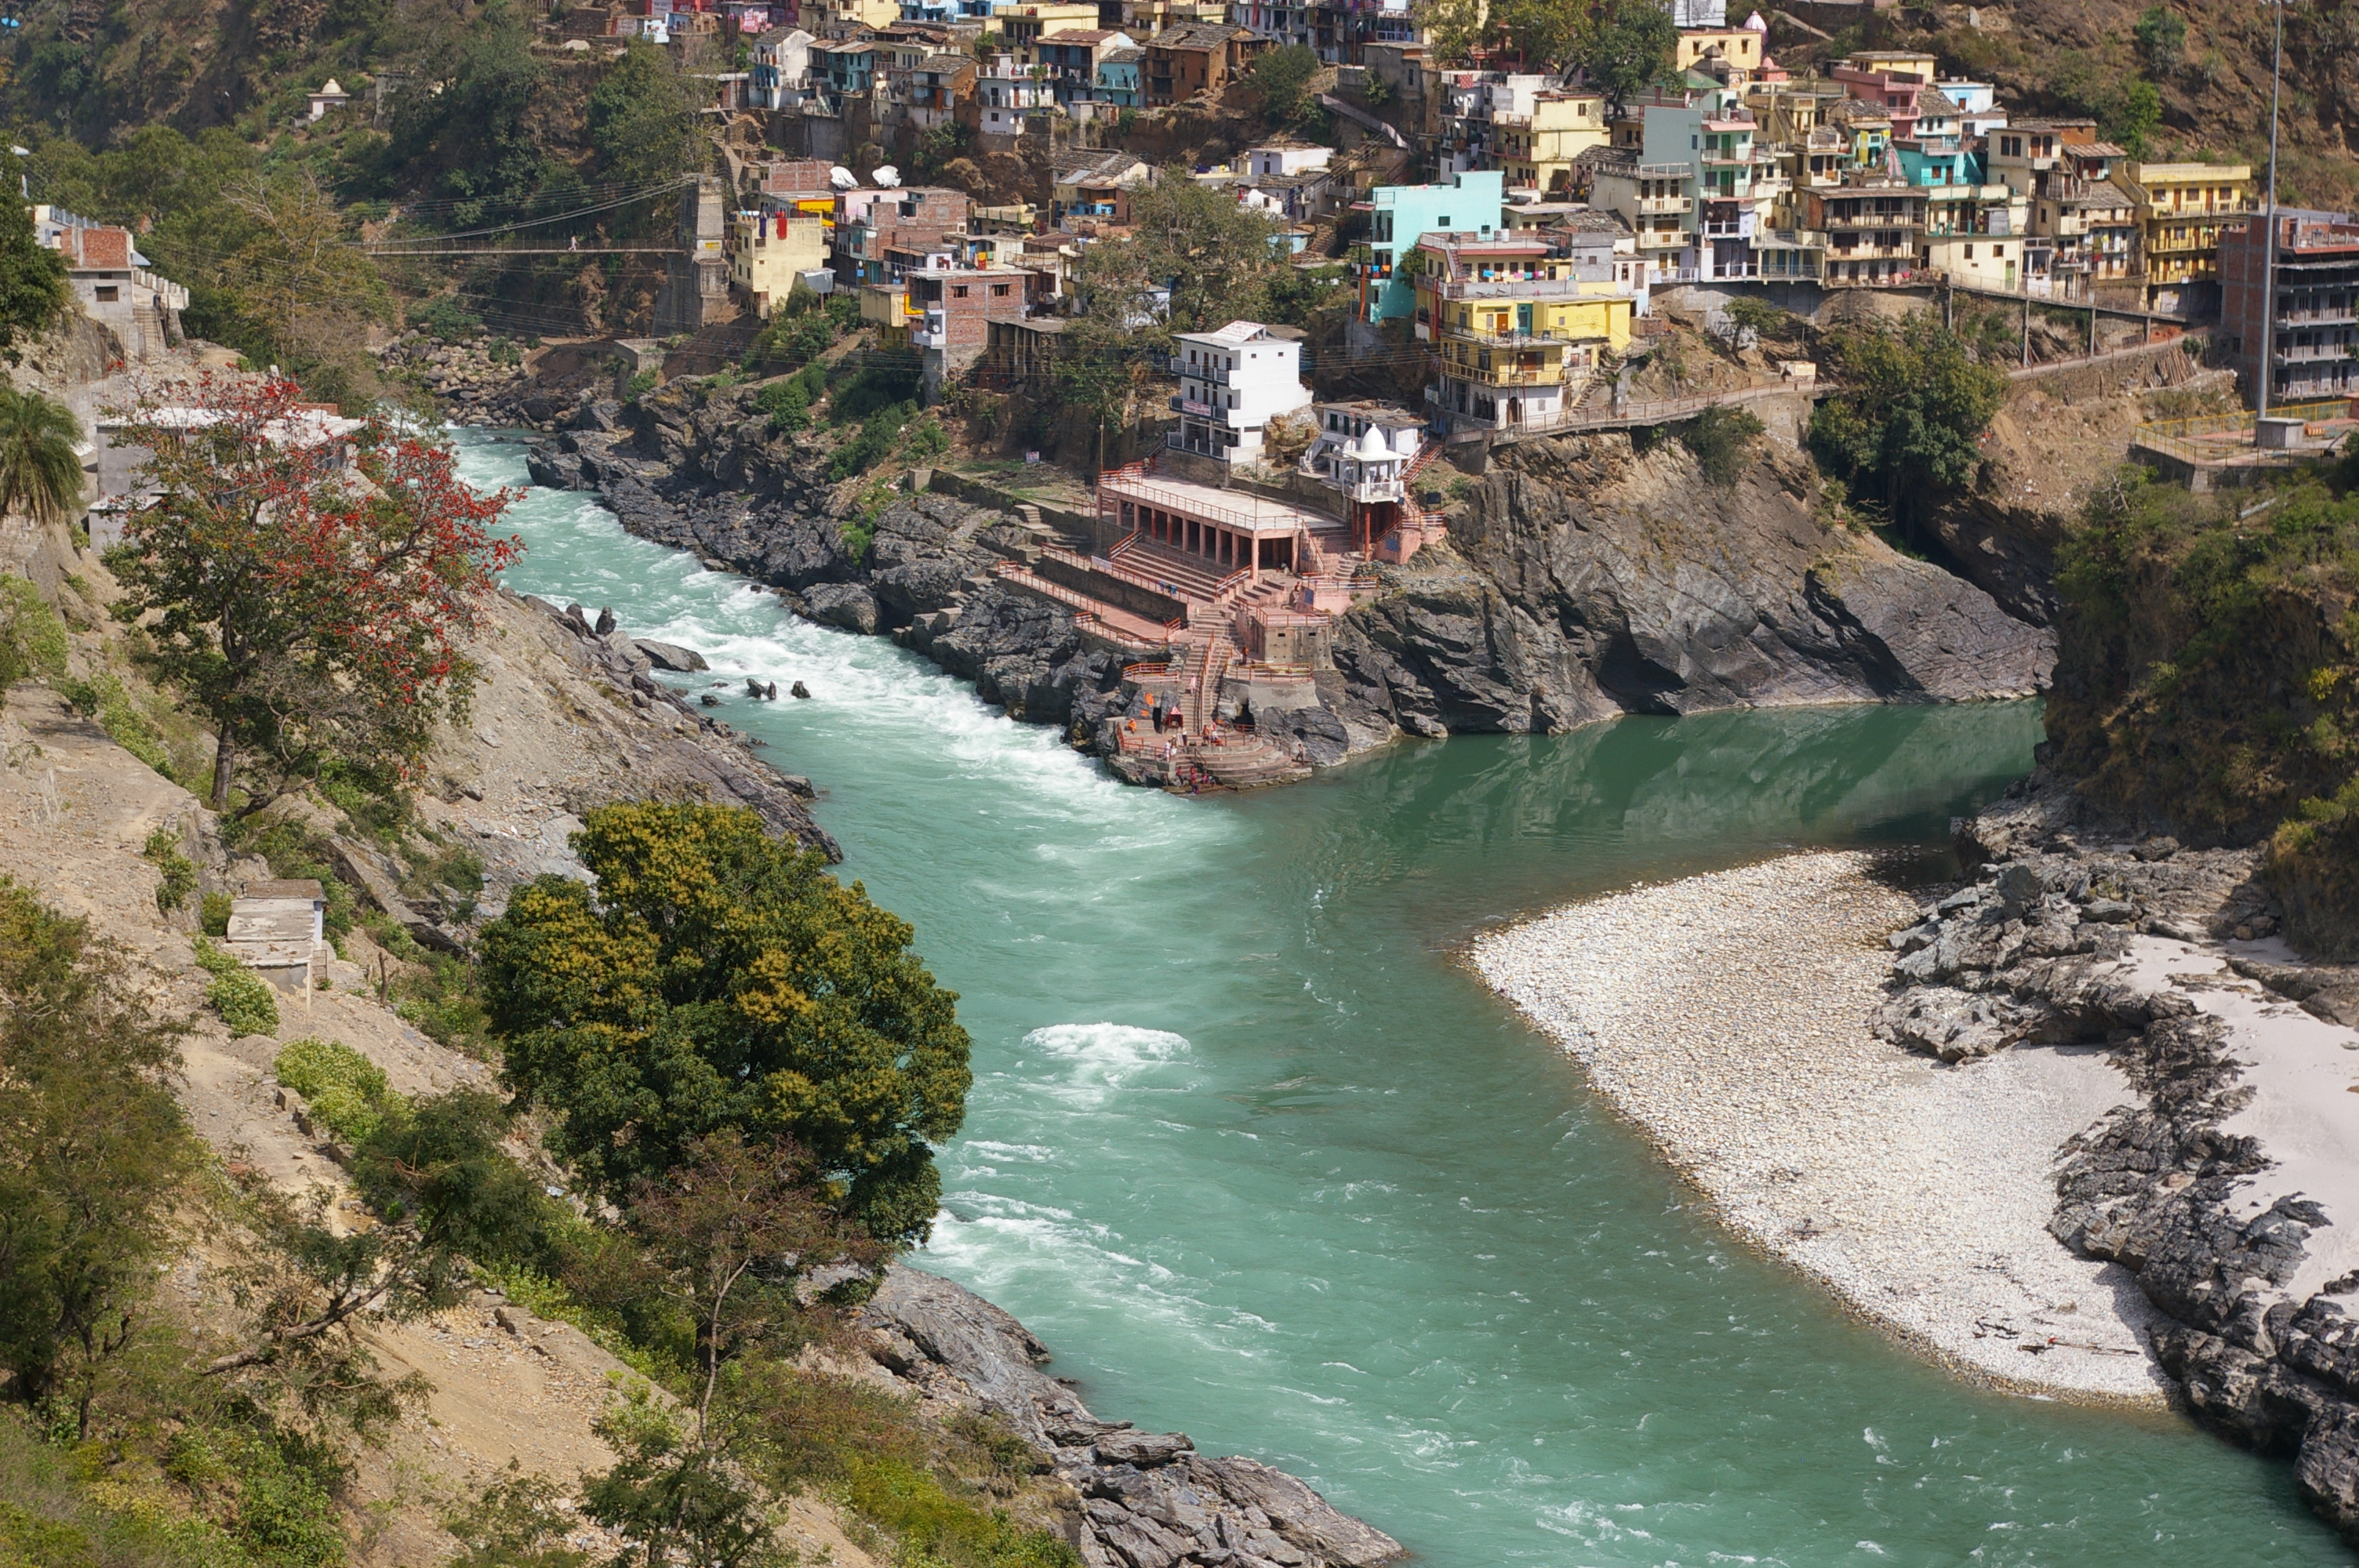
\includegraphics[width=\textwidth]{confluence.jpg}
\end{frame}

\begin{frame}
    \frametitle{Problemstellung}
    \small
    \begin{alignat*}{5}
           && p_1 &&     && && p_0 \\
        {\color{white}a +}&& 93  &&   {\color{white}b} &&{\color{white}=}&& 172 \\
        {\color{white}a +}&& 193 &&   {\color{white}b} &&{\color{white}=}&& 309 \\
        {\color{white}a +}&& 187 &&   {\color{white}b} &&{\color{white}=}&& 302 \\
        {\color{white}a +}&& 174 &&   {\color{white}b} &&{\color{white}=}&& 283 \\
        {\color{white}a +}&& 291 &&   {\color{white}b} &&{\color{white}=}&& 443 \\
        {\color{white}a +}&& 184 &&   {\color{white}b} &&{\color{white}=}&& 298 \\
        {\color{white}a +}&& 205 &&   {\color{white}b} &&{\color{white}=}&& 319 \\
        {\color{white}a +}&& 260 &&   {\color{white}b} &&{\color{white}=}&& 419 \\
        {\color{white}a +}&& 212 &&   {\color{white}b} &&{\color{white}=}&& 361 \\
        {\color{white}a +}&& 169 &&   {\color{white}b} &&{\color{white}=}&& 267 \\
        {\color{white}a +}&& 216 &&   {\color{white}b} &&{\color{white}=}&& 337 \\
        {\color{white}a +}&& 144 &&   {\color{white}b} &&{\color{white}=}&& 230
    \end{alignat*}
\end{frame}

\begin{frame}
    \centering
    \frametitle{Problemstellung}
    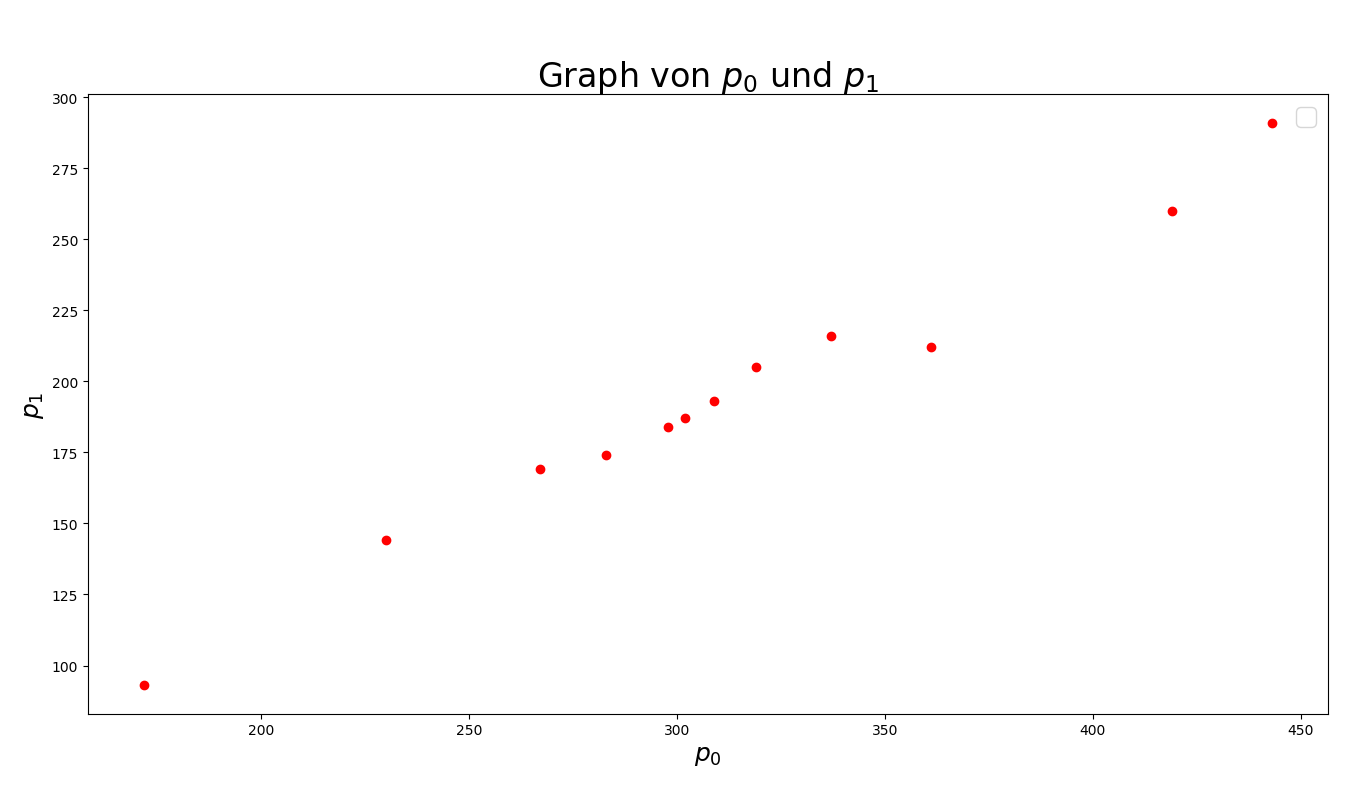
\includegraphics[width=\textwidth]{scatter.png}
\end{frame}

\begin{frame}
    \frametitle{Problemstellung}
    \small
    \begin{alignat*}{5}
           && p_1 &&     && && p_0 \\
        {\color{white}a +}&&                     93 &&   {\color{white}b} &&{\color{white}=}&&                    172 \\
        {\color{white}a +}&&                    193 &&   {\color{white}b} &&{\color{white}=}&&                    309 \\
        {\color{white}a +}&& {\color{lightgray}187} &&   {\color{white}b} &&{\color{white}=}&& {\color{lightgray}302} \\
        {\color{white}a +}&& {\color{lightgray}174} &&   {\color{white}b} &&{\color{white}=}&& {\color{lightgray}283} \\
        {\color{white}a +}&& {\color{lightgray}291} &&   {\color{white}b} &&{\color{white}=}&& {\color{lightgray}443} \\
        {\color{white}a +}&& {\color{lightgray}184} &&   {\color{white}b} &&{\color{white}=}&& {\color{lightgray}298} \\
        {\color{white}a +}&& {\color{lightgray}205} &&   {\color{white}b} &&{\color{white}=}&& {\color{lightgray}319} \\
        {\color{white}a +}&& {\color{lightgray}260} &&   {\color{white}b} &&{\color{white}=}&& {\color{lightgray}419} \\
        {\color{white}a +}&& {\color{lightgray}212} &&   {\color{white}b} &&{\color{white}=}&& {\color{lightgray}361} \\
        {\color{white}a +}&& {\color{lightgray}169} &&   {\color{white}b} &&{\color{white}=}&& {\color{lightgray}267} \\
        {\color{white}a +}&& {\color{lightgray}216} &&   {\color{white}b} &&{\color{white}=}&& {\color{lightgray}337} \\
        {\color{white}a +}&& {\color{lightgray}144} &&   {\color{white}b} &&{\color{white}=}&& {\color{lightgray}230}
    \end{alignat*}
\end{frame}

\begin{frame}
    \frametitle{Problemstellung}
    \small
    \begin{alignat*}{5}
           && p_1 &&     && && p_0 \\
        {\color{red}a} +&&                     93 &&   {\color{teal}b}    &&               =&&                    172 \\
        {\color{red}a} +&&                    193 &&   {\color{teal}b}    &&               =&&                    309 \\
        {\color{white}a +}&& {\color{lightgray}187} &&   {\color{white}b} &&{\color{white}=}&& {\color{lightgray}302} \\
        {\color{white}a +}&& {\color{lightgray}174} &&   {\color{white}b} &&{\color{white}=}&& {\color{lightgray}283} \\
        {\color{white}a +}&& {\color{lightgray}291} &&   {\color{white}b} &&{\color{white}=}&& {\color{lightgray}443} \\
        {\color{white}a +}&& {\color{lightgray}184} &&   {\color{white}b} &&{\color{white}=}&& {\color{lightgray}298} \\
        {\color{white}a +}&& {\color{lightgray}205} &&   {\color{white}b} &&{\color{white}=}&& {\color{lightgray}319} \\
        {\color{white}a +}&& {\color{lightgray}260} &&   {\color{white}b} &&{\color{white}=}&& {\color{lightgray}419} \\
        {\color{white}a +}&& {\color{lightgray}212} &&   {\color{white}b} &&{\color{white}=}&& {\color{lightgray}361} \\
        {\color{white}a +}&& {\color{lightgray}169} &&   {\color{white}b} &&{\color{white}=}&& {\color{lightgray}267} \\
        {\color{white}a +}&& {\color{lightgray}216} &&   {\color{white}b} &&{\color{white}=}&& {\color{lightgray}337} \\
        {\color{white}a +}&& {\color{lightgray}144} &&   {\color{white}b} &&{\color{white}=}&& {\color{lightgray}230}
    \end{alignat*}
\end{frame}

\begin{frame}
    \frametitle{Problemstellung}
    \small
    \begin{alignat*}{5}
           && p_1 &&     && && p_0 \\
        {\color{red}a} +&& 93  &&   {\color{teal}b} &&=&& 172 \\
        {\color{red}a} +&& 193 &&   {\color{teal}b} &&=&& 309 \\
        {\color{red}a} +&& 187 &&   {\color{teal}b} &&=&& 302 \\
        {\color{red}a} +&& 174 &&   {\color{teal}b} &&=&& 283 \\
        {\color{red}a} +&& 291 &&   {\color{teal}b} &&=&& 443 \\
        {\color{red}a} +&& 184 &&   {\color{teal}b} &&=&& 298 \\
        {\color{red}a} +&& 205 &&   {\color{teal}b} &&=&& 319 \\
        {\color{red}a} +&& 260 &&   {\color{teal}b} &&=&& 419 \\
        {\color{red}a} +&& 212 &&   {\color{teal}b} &&=&& 361 \\
        {\color{red}a} +&& 169 &&   {\color{teal}b} &&=&& 267 \\
        {\color{red}a} +&& 216 &&   {\color{teal}b} &&=&& 337 \\
        {\color{red}a} +&& 144 &&   {\color{teal}b} &&=&& 230
    \end{alignat*}
\end{frame}

\begin{frame}
    \frametitle{Problemstellung}
    \small
    \begin{alignat*}{5}
           && p_1 &&     && && p_0 \\
        1{\color{red}a} +&& 93  &&   {\color{teal}b} &&=&& 172 \\
        1{\color{red}a} +&& 193 &&   {\color{teal}b} &&=&& 309 \\
        1{\color{red}a} +&& 187 &&   {\color{teal}b} &&=&& 302 \\
        1{\color{red}a} +&& 174 &&   {\color{teal}b} &&=&& 283 \\
        1{\color{red}a} +&& 291 &&   {\color{teal}b} &&=&& 443 \\
        1{\color{red}a} +&& 184 &&   {\color{teal}b} &&=&& 298 \\
        1{\color{red}a} +&& 205 &&   {\color{teal}b} &&=&& 319 \\
        1{\color{red}a} +&& 260 &&   {\color{teal}b} &&=&& 419 \\
        1{\color{red}a} +&& 212 &&   {\color{teal}b} &&=&& 361 \\
        1{\color{red}a} +&& 169 &&   {\color{teal}b} &&=&& 267 \\
        1{\color{red}a} +&& 216 &&   {\color{teal}b} &&=&& 337 \\
        1{\color{red}a} +&& 144 &&   {\color{teal}b} &&=&& 230
    \end{alignat*}
\end{frame}

\begin{frame}
    \frametitle{Problemstellung}
    \small
    \begin{align*}
        \underbrace{
        \begin{pmatrix}
            1 &  93 \\
            1 & 193 \\
            1 & 187 \\
            1 & 174 \\
            1 & 291 \\
            1 & 184 \\
            1 & 205 \\
            1 & 260 \\
            1 & 212 \\
            1 & 169 \\
            1 & 216 \\
            1 & 144
        \end{pmatrix}
        }_A
        \underbrace{
        \begin{pmatrix}
            a \\ b
        \end{pmatrix}
        }_x
        =
        \underbrace{
        \begin{pmatrix}        
            172 \\
            309 \\
            302 \\
            283 \\
            443 \\
            298 \\
            319 \\
            419 \\
            361 \\
            267 \\
            337 \\
            230
        \end{pmatrix}
        }_v
    \end{align*}
\end{frame}

\begin{frame}
    \frametitle{Problemstellung}
    \small
    \begin{align*}
        \underbrace{
        \begin{pmatrix}
            1 &  93 \\
            1 & 193 \\
            1 & 187 \\
            1 & 174 \\
            1 & 291 \\
            1 & 184 \\
            1 & 205 \\
            1 & 260 \\
            1 & 212 \\
            1 & 169 \\
            1 & 216 \\
            1 & 144
        \end{pmatrix}
        }_A
        \underbrace{
        \begin{pmatrix}
            a \\ b
        \end{pmatrix}
        }_x
        {\color{red}\myeq}
        \underbrace{
        \begin{pmatrix}        
            172 \\
            309 \\
            302 \\
            283 \\
            443 \\
            298 \\
            319 \\
            419 \\
            361 \\
            267 \\
            337 \\
            230
        \end{pmatrix}
        }_v
    \end{align*}
\end{frame}

\begin{frame}
    \frametitle{Theorie}
    \begin{align*}
        ||Ax - b||_2
    \end{align*}
    {\color{white}Frage: Wie bestimmen wir \(x = (a, b)^T\), sodass die obige Gleichung minimal ist?}
    \begin{enumerate}
        \item {\color{white}Bestimme die QR-Zerlegung von \(A\). Also \(A = QR\).}
        \item {\color{white}Berechne \(z := Q^T v\). Definiere \(z_1\) als die ersten \(n\) Einträge (Breite von \(A\), hier \(n = 2\)) von \(z\).}
        \item {\color{white}Definiere \(R_1\) als die Matrix, die die ersten \(n \times n\) Einträge von \(R\) enthält.}
        \item {\color{white}Löse \(R_1 x = z_1\) durch Rückwärtseinsetzen.}
    \end{enumerate}
    {\color{white}Dann gilt: \(\text{min}||Ax - b||_2 = z_2\).}
\end{frame}

\begin{frame}
    \frametitle{Theorie}
    \begin{align*}
        ||Ax - b||_2
    \end{align*}
    Frage: Wie bestimmen wir \(x = (a, b)^T\), sodass die obige Gleichung minimal ist?
    \begin{enumerate}
        \item {\color{white}Bestimme die QR-Zerlegung von \(A\). Also \(A = QR\).}
        \item {\color{white}Berechne \(z := Q^T v\). Definiere \(z_1\) als die ersten \(n\) Einträge (Breite von \(A\), hier \(n = 2\)) von \(z\).}
        \item {\color{white}Definiere \(R_1\) als die Matrix, die die ersten \(n \times n\) Einträge von \(R\) enthält.}
        \item {\color{white}Löse \(R_1 x = z_1\) durch Rückwärtseinsetzen.}
    \end{enumerate}
    {\color{white}Dann gilt: \(\text{min}||Ax - b||_2 = z_2\).}
\end{frame}

\begin{frame}
    \frametitle{Theorie}
    \begin{align*}
        ||Ax - b||_2
    \end{align*}
    Frage: Wie bestimmen wir \(x = (a, b)^T\), sodass die obige Gleichung minimal ist?
    \begin{enumerate}
        \item Bestimme die QR-Zerlegung von \(A\). Also \(A = QR\).
        \item {\color{white}Berechne \(z := Q^T v\). Definiere \(z_1\) als die ersten \(n\) Einträge (Breite von \(A\), hier \(n = 2\)) von \(z\).}
        \item {\color{white}Definiere \(R_1\) als die Matrix, die die ersten \(n \times n\) Einträge von \(R\) enthält.}
        \item {\color{white}Löse \(R_1 x = z_1\) durch Rückwärtseinsetzen.}
    \end{enumerate}
    {\color{white}Dann gilt: \(\text{min}||Ax - b||_2 = z_2\).}
\end{frame}

\begin{frame}
    \frametitle{Theorie}
    \begin{align*}
        ||Ax - b||_2
    \end{align*}
    Frage: Wie bestimmen wir \(x = (a, b)^T\), sodass die obige Gleichung minimal ist?
    \begin{enumerate}
        \item Bestimme die QR-Zerlegung von \(A\). Also \(A = QR\).
        \item Berechne \(z := Q^T v\). Definiere \(z_1\) als die ersten \(n\) Einträge (Breite von \(A\), hier \(n = 2\)) von \(z\).
        \item {\color{white}Definiere \(R_1\) als die Matrix, die die ersten \(n \times n\) Einträge von \(R\) enthält.}
        \item {\color{white}Löse \(R_1 x = z_1\) durch Rückwärtseinsetzen.}
    \end{enumerate}
    {\color{white}Dann gilt: \(\text{min}||Ax - b||_2 = z_2\).}
\end{frame}

\begin{frame}
    \frametitle{Theorie}
    \begin{align*}
        ||Ax - b||_2
    \end{align*}
    Frage: Wie bestimmen wir \(x = (a, b)^T\), sodass die obige Gleichung minimal ist?
    \begin{enumerate}
        \item Bestimme die QR-Zerlegung von \(A\). Also \(A = QR\).
        \item Berechne \(z := Q^T v\). Definiere \(z_1\) als die ersten \(n\) Einträge (Breite von \(A\), hier \(n = 2\)) von \(z\).
        \item Definiere \(R_1\) als die Matrix, die die ersten \(n \times n\) Einträge von \(R\) enthält.
        \item {\color{white}Löse \(R_1 x = z_1\) durch Rückwärtseinsetzen.}
    \end{enumerate}
    {\color{white}Dann gilt: \(\text{min}||Ax - b||_2 = z_2\).}
\end{frame}

\begin{frame}
    \frametitle{Theorie}
    \begin{align*}
        ||Ax - b||_2
    \end{align*}
    Frage: Wie bestimmen wir \(x = (a, b)^T\), sodass die obige Gleichung minimal ist?
    \begin{enumerate}
        \item Bestimme die QR-Zerlegung von \(A\). Also \(A = QR\).
        \item Berechne \(z := Q^T v\). Definiere \(z_1\) als die ersten \(n\) Einträge (Breite von \(A\), hier \(n = 2\)) von \(z\).
        \item Definiere \(R_1\) als die Matrix, die die ersten \(n \times n\) Einträge von \(R\) enthält.
        \item Löse \(R_1 x = z_1\) durch Rückwärtseinsetzen.
    \end{enumerate}
    {\color{white}Dann gilt: \(\text{min}||Ax - b||_2 = z_2\).}
\end{frame}

\begin{frame}
    \frametitle{Theorie}
    \begin{align*}
        ||Ax - b||_2
    \end{align*}
    Frage: Wie bestimmen wir \(x = (a, b)^T\), sodass die obige Gleichung minimal ist?
    \begin{enumerate}
        \item Bestimme die QR-Zerlegung von \(A\). Also \(A = QR\).
        \item Berechne \(z := Q^T v\). Definiere \(z_1\) als die ersten \(n\) Einträge (Breite von \(A\), hier \(n = 2\)) von \(z\).
        \item Definiere \(R_1\) als die Matrix, die die ersten \(n \times n\) Einträge von \(R\) enthält.
        \item Löse \(R_1 x = z_1\) durch Rückwärtseinsetzen.
    \end{enumerate}
    Dann gilt: \(\text{min}||Ax - b||_2 = ||z_2||_2\).
\end{frame}

\begin{frame}
    \centering
    \frametitle{Theorie}
    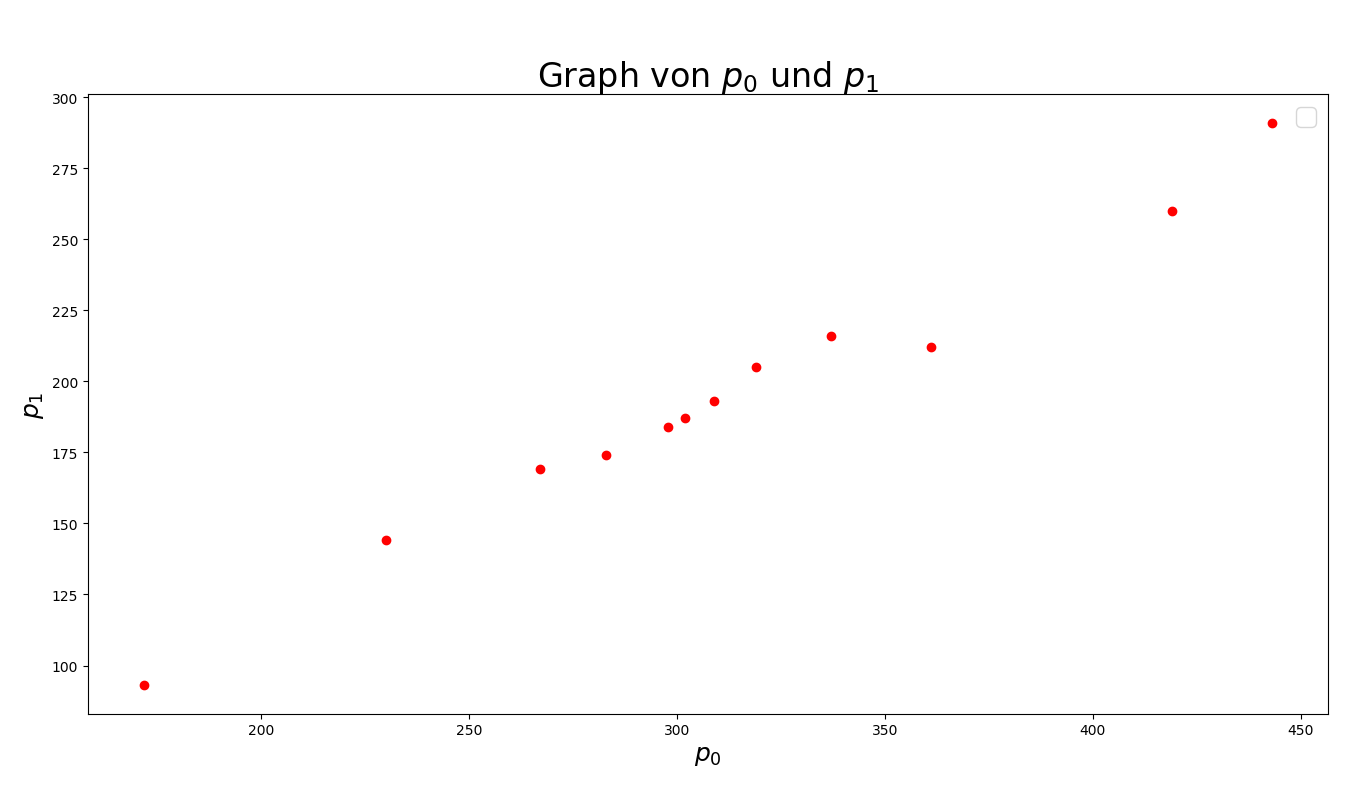
\includegraphics[width=\textwidth]{scatter.png}
\end{frame}

\begin{frame}
    \frametitle{Theorie}
    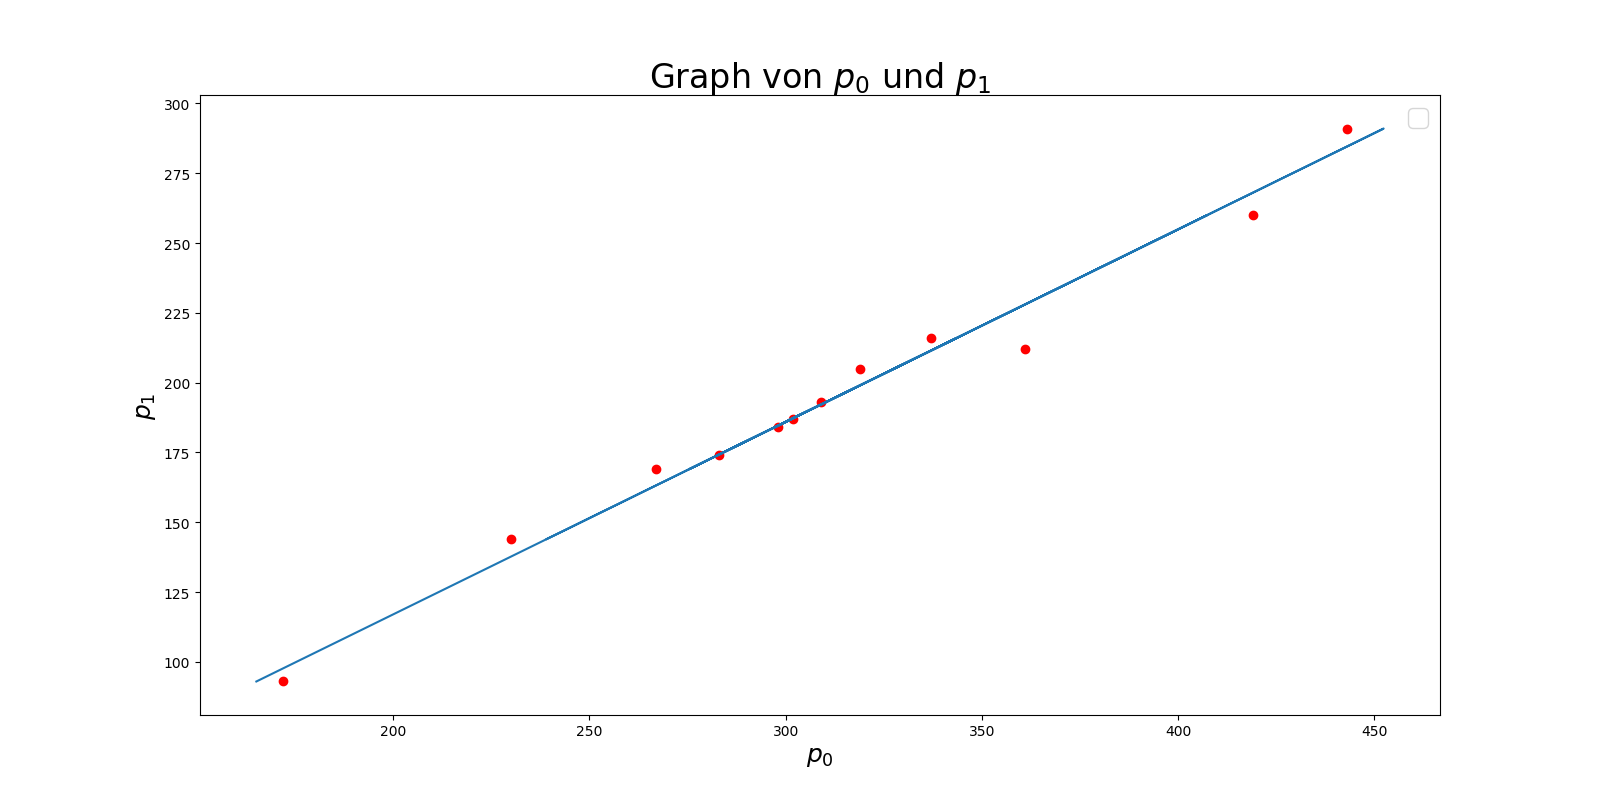
\includegraphics[width=\textwidth]{plot.png}
\end{frame}

\begin{frame}
    \frametitle{Theorie}
    \begin{center}
        \begin{tabular}{ c c c }
            $p_0$ & $p_1$ & $p_2$ \\
            \hline
            172 & 93 & 120 \\
            309 & 193 & 258 \\
            302 & 187 & 255 \\
            283 & 174 & 238 \\
            443 & 291 & 317 \\
            298 & 184 & 246 \\
            319 & 205 & 265 \\
            419 & 260 & 304 \\
            361 & 212 & 292 \\
            267 & 169 & 242 \\
            337 & 216 & 272 \\
            230 & 144 & 191
        \end{tabular}
    \end{center}    
\end{frame}

\begin{frame}
    \frametitle{Theorie}
    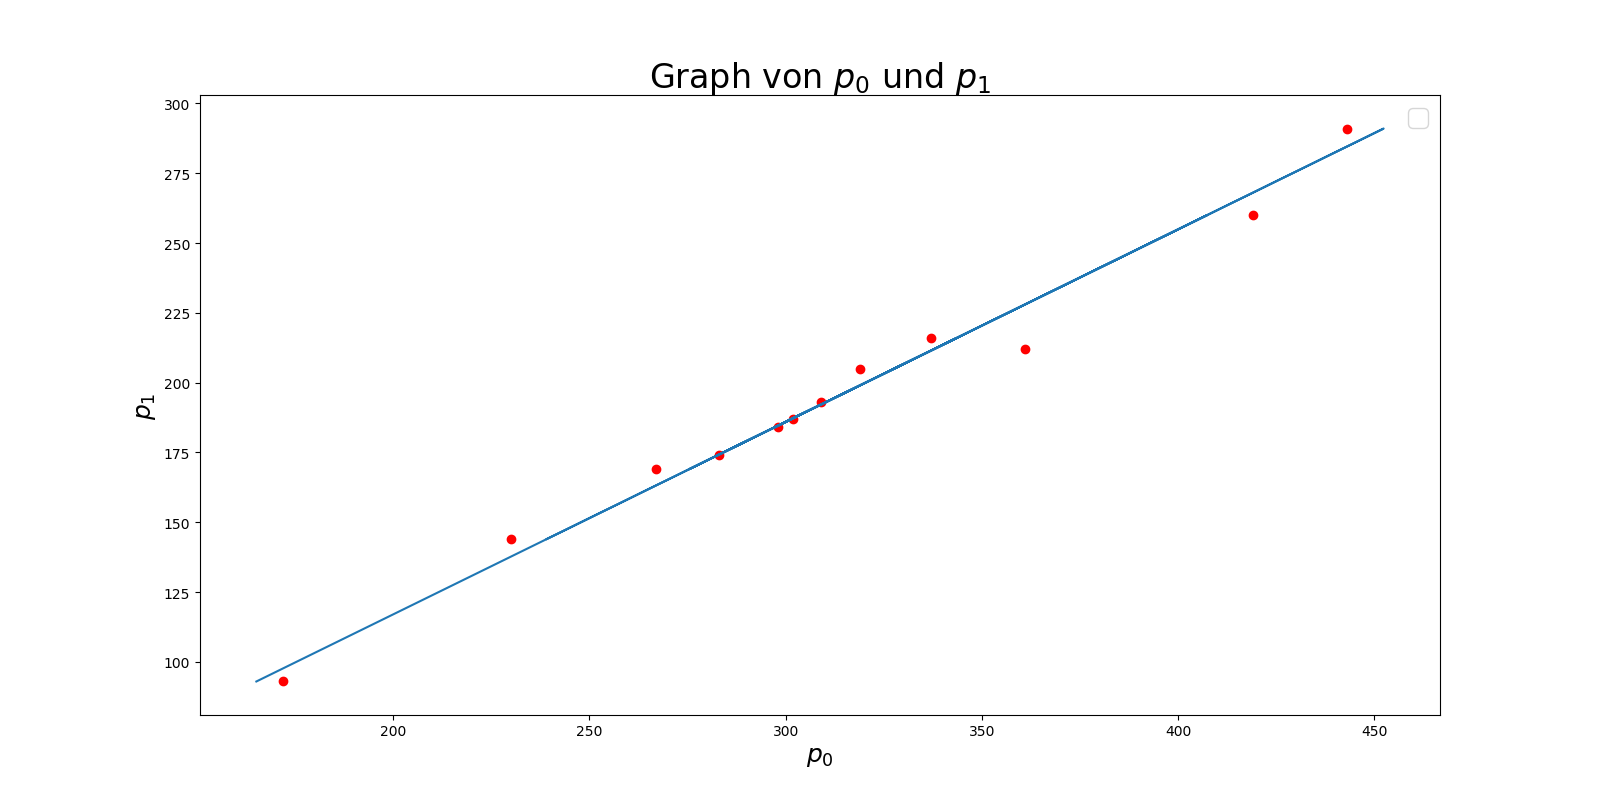
\includegraphics[width=\textwidth]{plot.png}
    
    Kondition: \(A = 74.26\), \(A^T A = 5514.75\)

    Residuum: 32.90 (ohne \(p_2\)), 32.09 (mit \(p_2\))
\end{frame}

\begin{frame}
Hier wurde nur die ersten 6 Werte betrachtet.

\frametitle{Experimente}
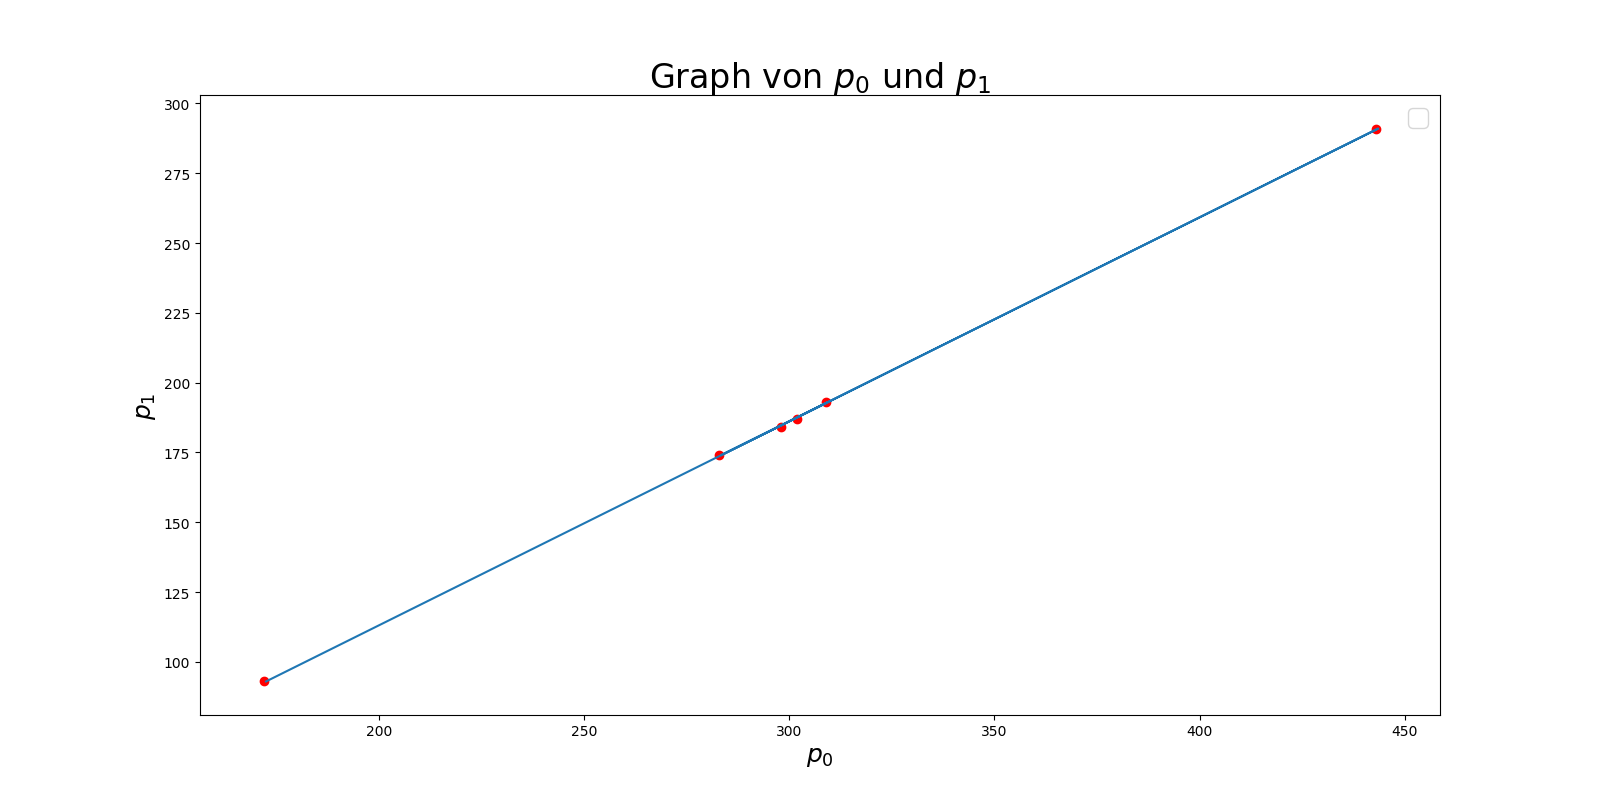
\includegraphics[width=\textwidth]{plot1.png}

Kondition: $A = 72.47$, $A^T A = 5252.05$

Residuum: 1.54 (ohne $p_2$), 1.26 (mit $p_2$)
\end{frame}

\begin{frame}
Hier wurden die letzten 2 Werte (von 12) stark verändert.

\frametitle{Experimente}
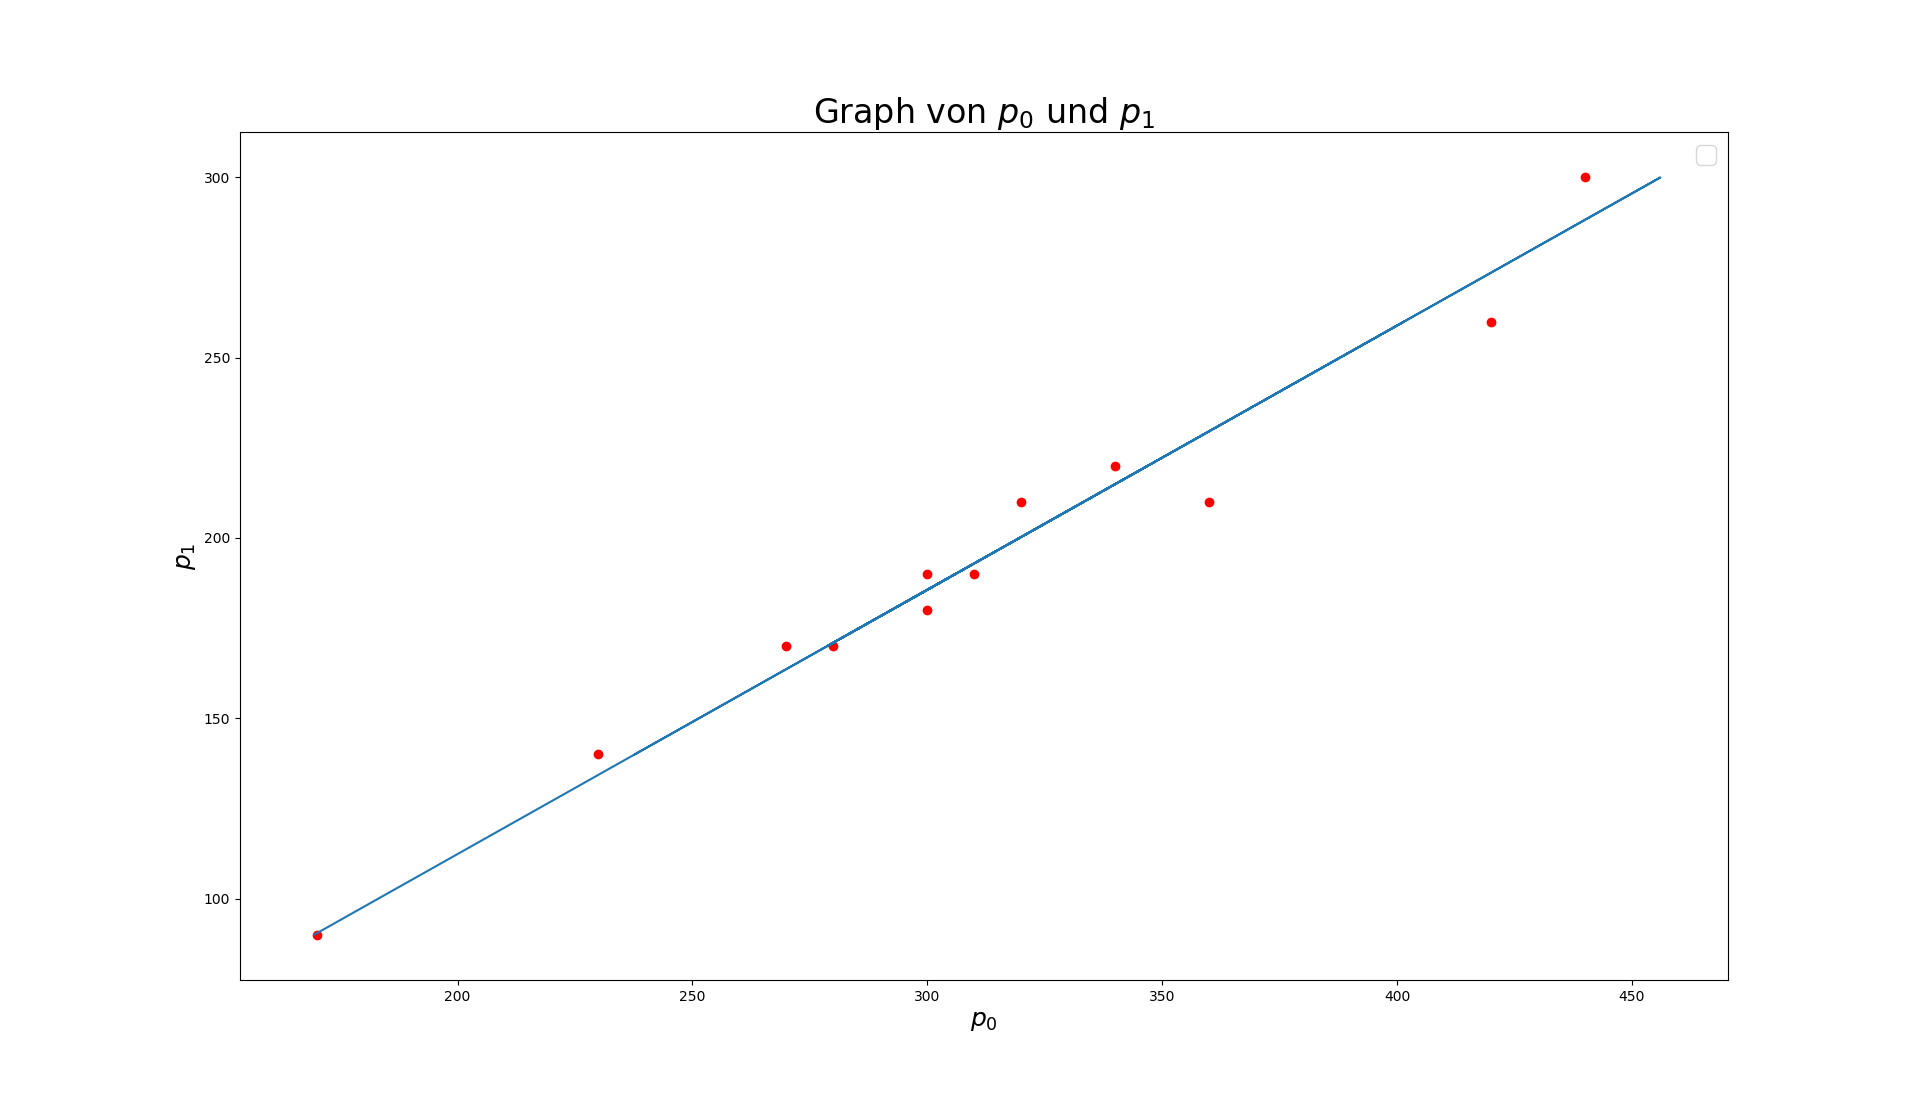
\includegraphics[width=\textwidth]{plot2.png}

Kondition: $A = 29.76$, $A^T A = 887.15$

Residuum: 324.40 (ohne $p_2$), 211.25 (mit $p_2$)
\end{frame}


\begin{frame}
    \frametitle{Zusammenfassung}
    
    \begin{itemize}
    
    \item {\color{white}Je weniger Werte desto kleiner das Residuum, aber wahrscheinlich wird das Modell zur Darstellung von physikalischen Phänomene inakkurater.}
    \item {\color{white}Sollten sich einige Werte sich stark von anderen unterscheiden, sollte man in Betracht ziehen diese Werte zu ignorieren. (Möglicherweise sollte ein Algorithmus benutzt werden, die eine Gewichtung den Werten zuweist.)}
    \end{itemize}
    
\end{frame}


\begin{frame}
\frametitle{Zusammenfassung}

\begin{itemize}

\item Je weniger Werte desto kleiner das Residuum, aber wahrscheinlich wird das Modell zur Darstellung von physikalischen Phänomene inakkurater. 
\item {\color{white}Sollten sich einige Werte sich stark von anderen unterscheiden, sollte man in Betracht ziehen diese Werte zu ignorieren. (Möglicherweise sollte ein Algorithmus benutzt werden, die eine Gewichtung den Werten zuweist.)}
\end{itemize}

\end{frame}

\begin{frame}
    \frametitle{Zusammenfassung}
    
    \begin{itemize}
    
    \item Je weniger Werte desto kleiner das Residuum, aber wahrscheinlich wird das Modell zur Darstellung von physikalischen Phänomene inakkurater. 
    \item Sollten sich einige Werte sich stark von anderen unterscheiden, sollte man in Betracht ziehen diese Werte zu ignorieren. (Möglicherweise sollte ein Algorithmus benutzt werden, die eine Gewichtung den Werten zuweist.)
    \end{itemize}
    
\end{frame}


\begin{frame}
\frametitle{Literatur}
\begin{enumerate}

\item \textit{Numerische Lineare Algebra}, Prof. Dr. Caren Tischendorf
\item Titelbild Quelle: \textit{Wikipedia}, https://en.wikipedia.org/wiki/Confluence

\end{enumerate}

\end{frame}


\end{document}